\documentclass{article}
\usepackage[utf8]{inputenc}
\usepackage[spanish]{babel}
\usepackage{listings}
\usepackage{graphicx}
\graphicspath{ {images/} }
\usepackage{cite}

\begin{document}

\begin{titlepage}
    \begin{center}
        \vspace*{1cm}
            
        \Huge
        \textbf{trabajo de investigacion}
        \vspace{0.5cm}
        \LARGE
        memoria en las computadoras
            
        \vspace{1.5cm}
            
        \textbf{Santiago Pereira Ramirez}
            
        \vfill
            
        \vspace{0.8cm}
            
        \Large
        Despartamento de Ingeniería Electrónica y Telecomunicaciones\\
        Universidad de Antioquia\\
        Medellín\\
        Septiembre de 2020
            
    \end{center}
\end{titlepage}

\tableofcontents

\section{Introduccion}
durante mucho tiempo se ha pensado que programar es mucho mas que  escribir codigo, en gran parte no deberia ser asi,ni mucho menos pensado.en la programacion para programar en un buen sentido de la palabra se debe de tener aspectos tales como la comprension y calidad del algoritmo que vamos a implementar,tener diferentes capacidades de comunicacion 
y formas de trabajar en equipo,asi como tener la disciplina y el empeño para realizar los diferentes trabajos asignados .Pero algo que es de sumamente importancia.
No solo al programar sino tambien en cualquier otro trabajo en el mundo el cual es conocer la herramien de trabajo y como lo que haremos influir en los dintintos 
tipos de dispositivos, a continuacion mostraremos aspectos muy importantes sobre la memoria, algo mas alla de guardar.

\section{Sección de contenido} \label{contenido}
    \subsection{Qué es la memoria de un computador?}
    Podemos definir la memoria en un contexto general, podriamos decir que es el proceso por el cual la memoria tiene capacidad mental que posibilita a un sujeto registrar, conservar y evocar las experiencias\cite{hipocampo}, y si volvemos a leer de nuevo, podemos plantear que esta idea no se aleja mucho de la logica con la cual es programado un computador, aunque sin apegarnos a esto y ademas profundizando, la memoria en el computador tiene un proceso complejo y que para algunos tiene una ventaja sobre los humanos, alguna de estas como la velocidad, rapidez y eficiencia.
    
    asi, la memoria en el computador cumple un papel fundamental para el buen funcionamiento del mismo  ya que se trata del dispositivo donde se almacena temporalmente toda la información con la que trabajan los microprocesadores para procesarla y devolver los resultados que los usuarios que la requieren.

    \begin{figure}[h]
    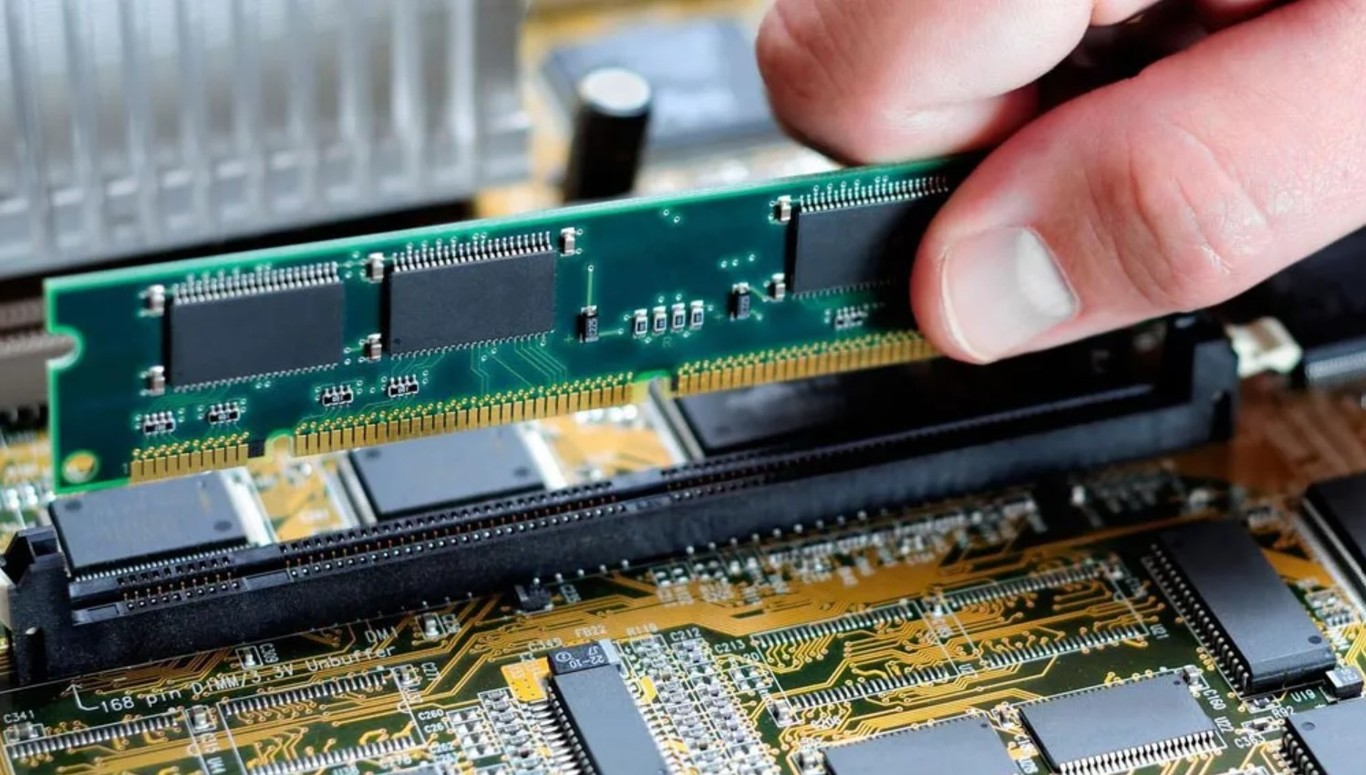
\includegraphics[width=6 cm]{imagenes/tipo_memoria.jpg}
    \centering
    \caption{foto memoria ram}
    \label{fig:tipo_memoria}
    \end{figure}

    Por otra parte podriamos decir que el termino de memoria es una taquigrafia(Técnica de escritura en la que se utilizan ciertos signos y abreviaturas especiales para poder transcribir todo lo que dice alguien a la misma velocidad a la que habla.) para la memoria fisica que se refiere a los chips que son capaces de llevar a cabo datos del computador.
    
    \subsection{Tipos de memoria}
    En las computadoras hay diferentes tipos de memoria, unas mas rapidaz que otras pero todas iguales de importantes y todas necesarias para el correcto funcionamiento, por ejemplo hoy en dia los microprocesadores cada vez son mas eficientes y veloces, capaces de procesar miles de millones de ciclos por segundo,po ende son capaces de procesar 
    miles de millones de bytes por segundo, por este motivo deben de tener dispositivos de almacenamiento tempor que puedan seguir el trabajo ya que si no fuera asise tendria que parar para cada informacion que llegue.
        \subsubsection{La memoria RAM}
        La memoria RAM es el tipo de memoria mas importante que tiene el computador,en este tipo de memoria se puede acceder desde cualquier espacio , mo importa si dirreccion o la posicion. Las siglas RAM significan ( Random Access Memory o memoria de acceso aleatorio)
    \subsection{¿Como se debe de gestionar una memoria en un computador?}
    \subsection{Qué hace que una memoria sea más rápida que otra y porque esto es importante?}
    


\begin{lstlisting}

\end{lstlisting}

(\ref{contenido})

\section{Conclusión} \label{conclulsion}

\bibliographystyle{IEEEtran}
\bibliography{references}

\end{document}
